% VLDB template version of 2020-08-03 enhances the ACM template, version 1.7.0:
% https://www.acm.org/publications/proceedings-template
% The ACM Latex guide provides further information about the ACM template

\documentclass[]{article}

\usepackage[a4paper,width=160mm,top=25mm,bottom=25mm]{geometry}

\usepackage{import}

\usepackage{subfig}
\usepackage{float}
\usepackage{graphicx}
\usepackage{hyperref}

\hypersetup{
	colorlinks,
	breaklinks,
    urlcolor=[rgb]{0,0.5,0.5},
    linkcolor=[rgb]{0,0.5,0.5}
}

\usepackage{indentfirst}

\rmfamily

\title{COEN6311 Deliverable 2: System Modeling and Design \\ GroupSuper}

\author{Ding Li 40160073 \\ Zerui Wang 40177315 \\ Jun Huang 40168167}
% \author{Zerui Wang 40177315}
% \author{Jun Huang 40168167}

\begin{document}

\maketitle

\linespread{1.2}
\selectfont

\section{Introduction}
This delivery includes a description of our process of following the Agile development process,
defining the RoadMap using the Jira management tool, performing requirements segmentation and relating user stories.
Also define 3 Sprints for development. It also includes a documentation section, defining the use case,
system architecture, modelling and designing ( Class Diagram, Activity Diagram, Sequence Diagram, Statement Diagram).
Also included is our Web UI design section.
At the end of the article, after revisiting the UI design,
we selected a new task as required and repeated the requirement section, having planned new milestones.


\section{Agile development process}

\textbf{Team Setup:} As a three members team, we define the roles of [Product Owner]
\textit{Jun Huang} and [Scrum Master] will be a shift between \textit{Zerui Wang} and \textit{Din Li}.
We use JIRA as our management tool,
the whole roadmap for the project is shown in Figure \ref{fig:roadmap}.

\begin{figure*}[htp]
	\centering
	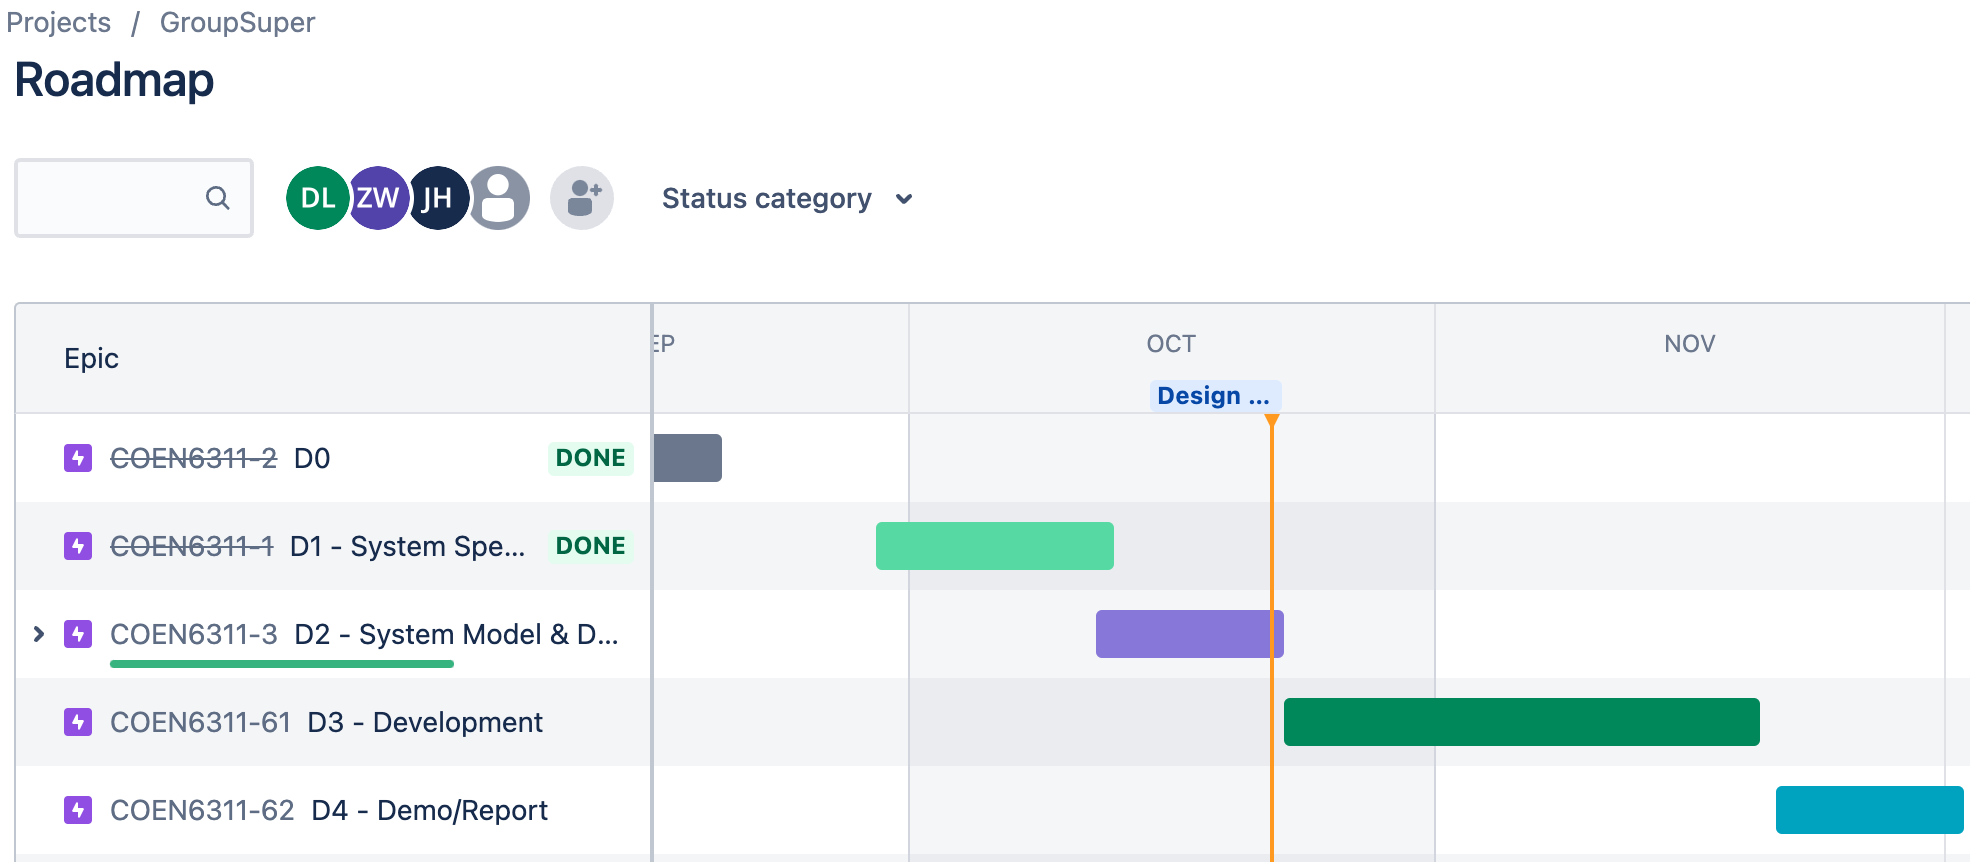
\includegraphics[width=0.8\textwidth]{./img/JiraRoadmap.png}
	\caption{Roadmap - JIRA Management Tool}
	\label{fig:roadmap}
\end{figure*}

\textbf{Associate user stories to sub-requirements:}
Previous deliverable we define three user stories and 7 sub-requirements.
They are associated to each other by JIRA linked issues feature.
Figure \ref{fig:subreq_example} gives an example that we connect User Story 2 Lucy
to the ICDE Record Capture and Access module in sub-requirement 4 and Authorized API Module in sub-requirement 5.
The full sub-requirement assignments are listed in our Jira panel:

\url{https://youyinnn.atlassian.net/jira/software/projects/COEN6311/boards/2/backlog}.

\begin{figure*}[htp]
	\centering
	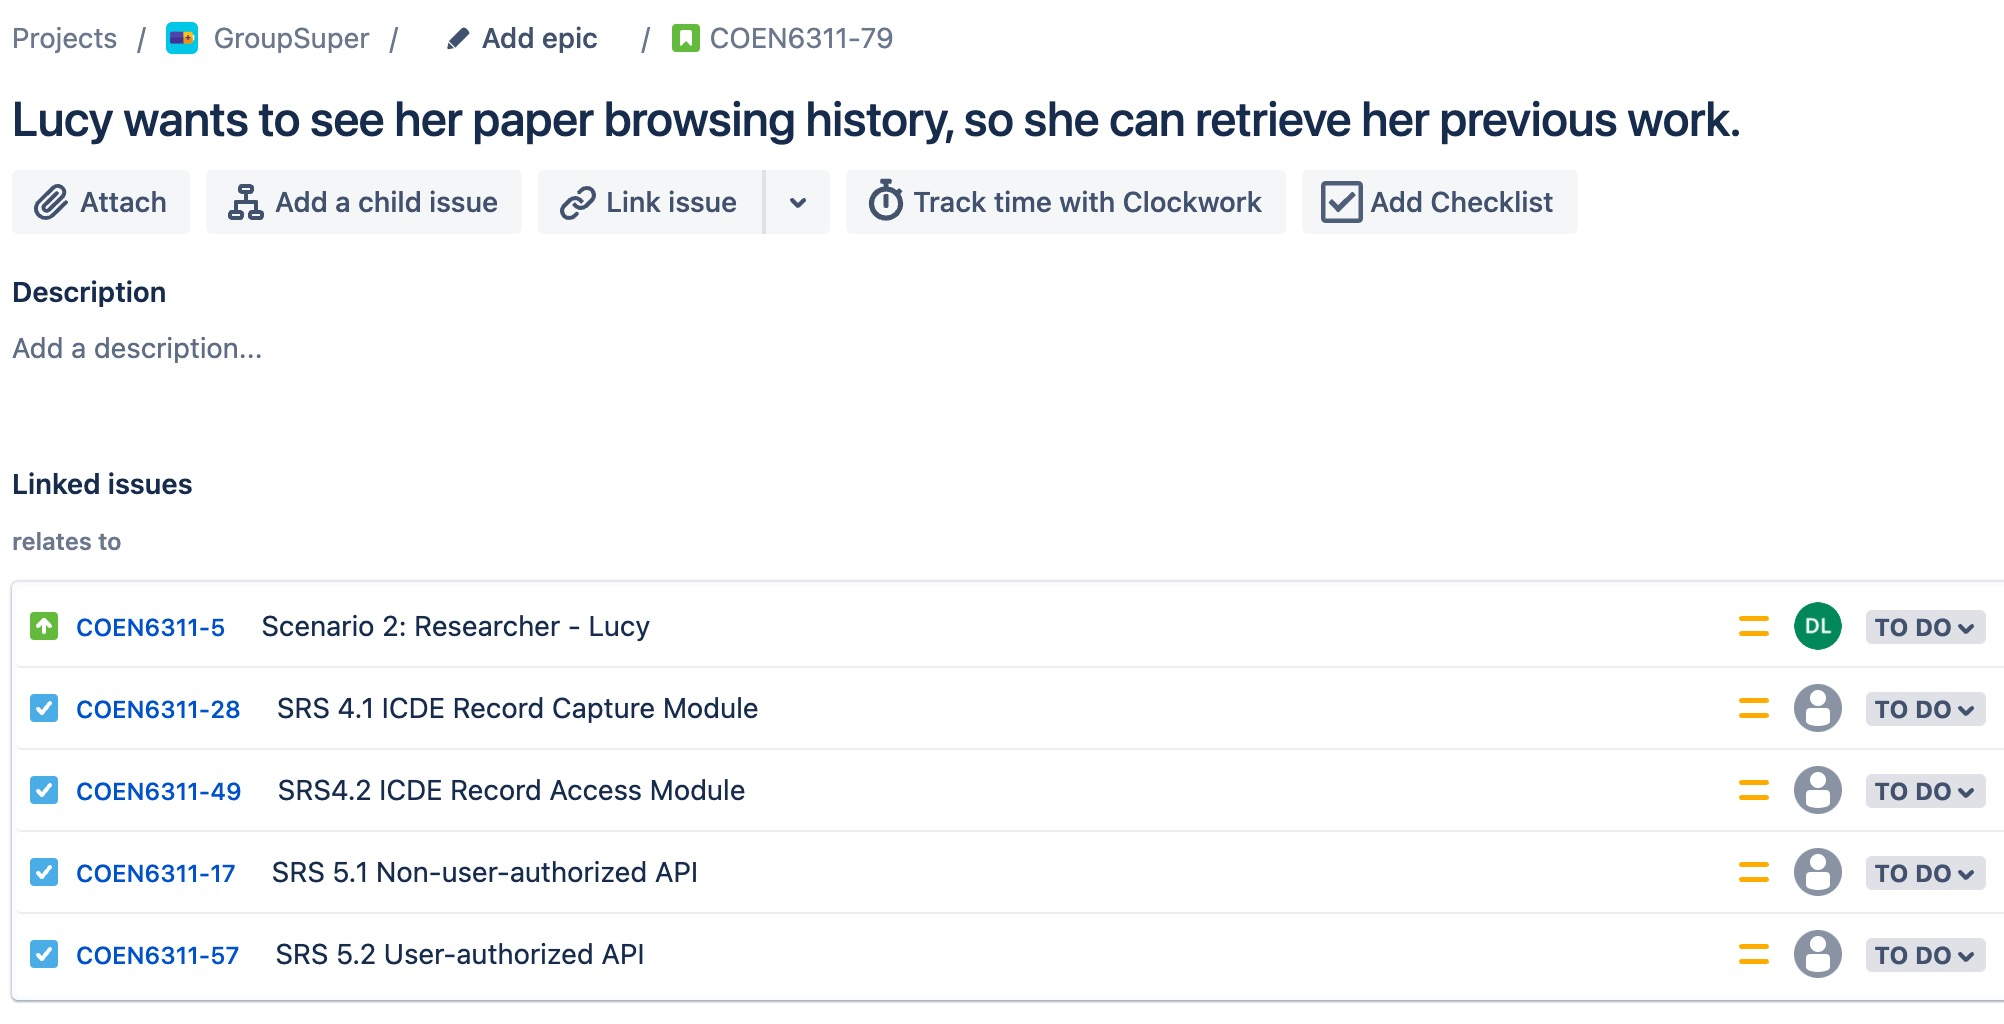
\includegraphics[width=0.8\textwidth]{./img/subreq_example.jpeg}
	\caption{An example of associating user stories to sub-req}
	\label{fig:subreq_example}
\end{figure*}

\textbf{Define tasks and priority under each requirement: }Tasks are deployed under each sub-requirement to be finished. We also separate different Dev Sprints to accomplish the whole project. Dev Sprint 1 includes Sub-requirements 1 \& 2 that involve login, log out and information management system. Dev Sprint 2 includes sub-requirements 3 \& 4 \& 5 that contains ICDE process and the authorized API. Dev Sprint 3 includes sub-requirements 6 \& 7 mainly for the team management service. Figure \ref{fig:devsprint} gives an example that how we add tasks under the sub-requirements defined earlier. The UML diagrams modelling and designing tasks for the whole system are also considered as a Sprint.

\begin{figure*}[htp]
	\centering
	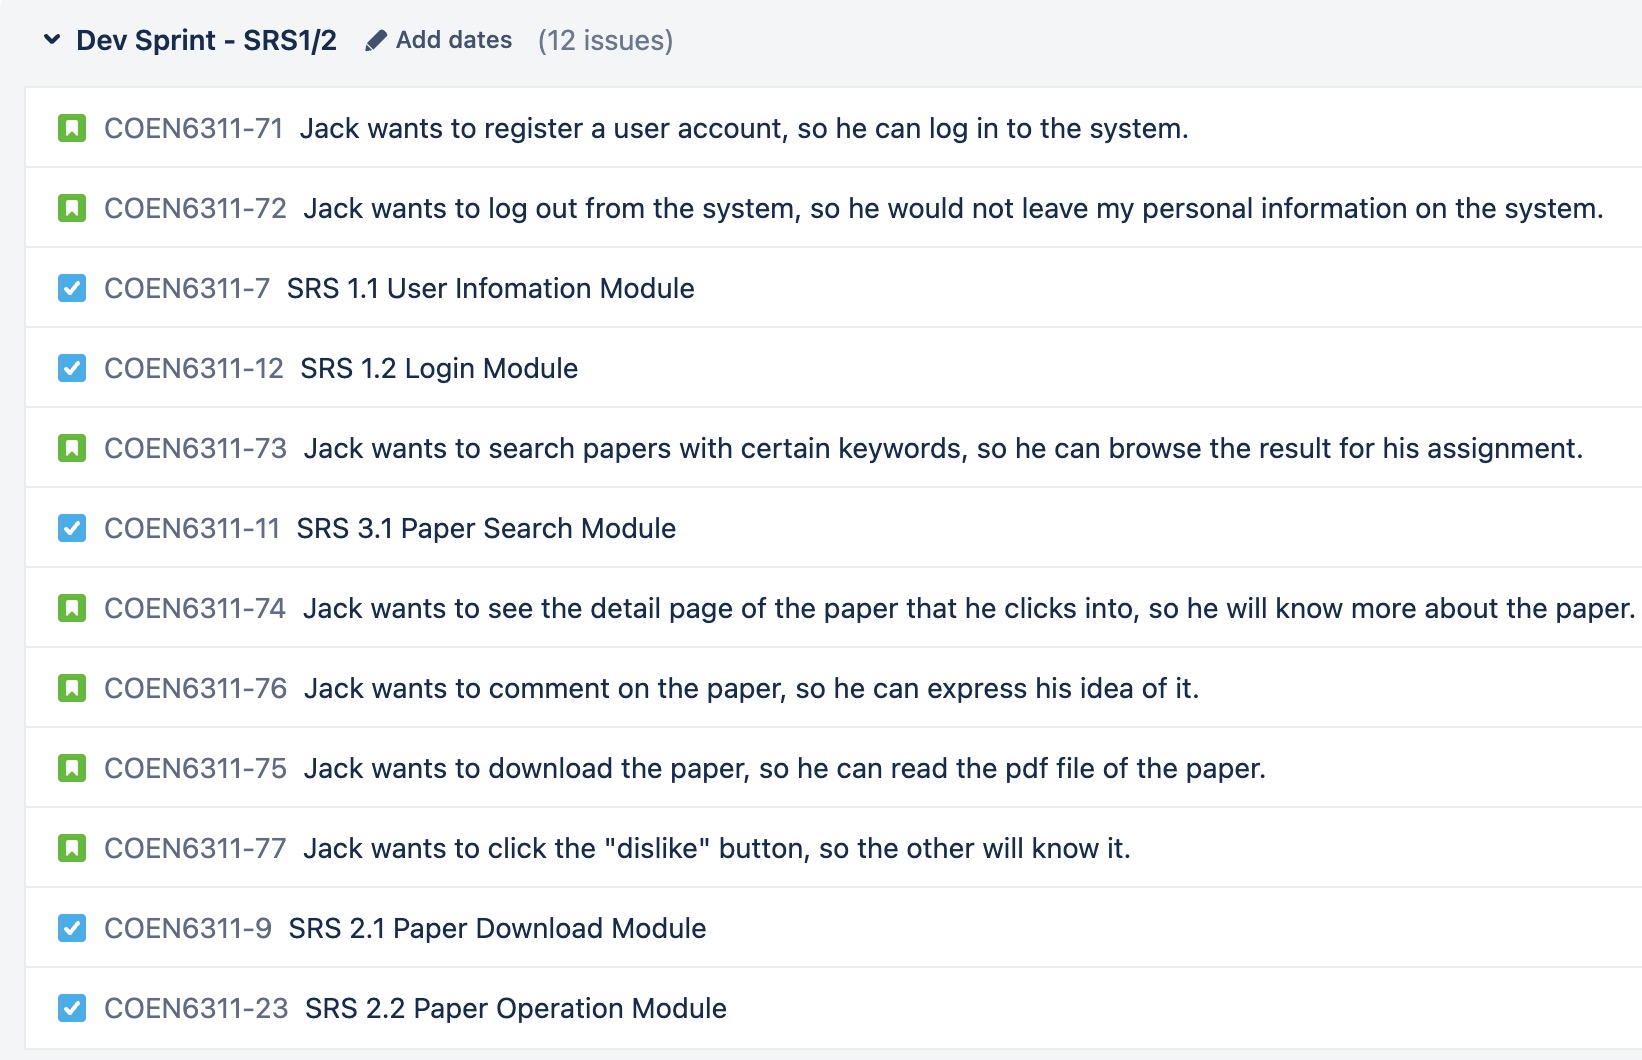
\includegraphics[width=0.8\textwidth]{./img/devsprint.jpeg}
	\caption{An example of defining tasks under each Sprint}
	\label{fig:devsprint}
\end{figure*}

\section{Revising and Modelling.}
This section includes the modelling and designing both overall level and user/system requirements level.

\subsection{Revise the context/external description}

\textbf{Overall Use Cases: }  The overall use case is shown as Figure \ref{fig:oucs}.

\begin{figure*}[!ht]
	\centering
	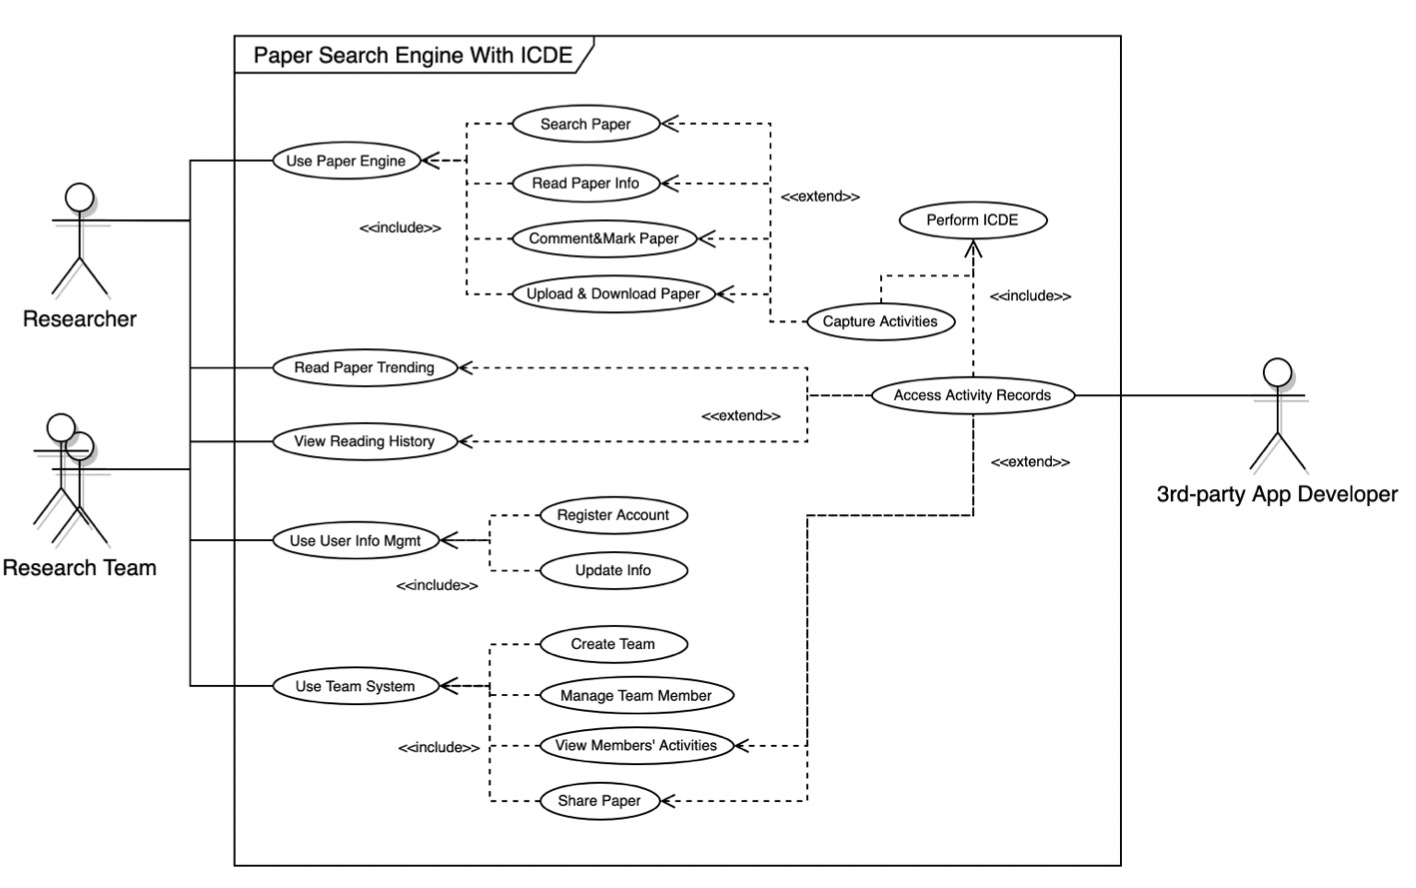
\includegraphics[width=0.8\textwidth]{./img/Figure_overall-use-cases.jpg}
	\caption{Overall Use Cases}
	\label{fig:oucs}
\end{figure*}

\textbf{Use case Diagrams: }  According to the various sub-requirements level,
we specify the use cases as follows of user requirements and system requirements level,
which are shown in different subgraphs of Fig. \ref{fig:subusercases-1} and Fig. \ref{fig:subusercases-2}.

\begin{figure*}[!ht]
	\centering
	\subfloat[Use Case Sub-Req 1]{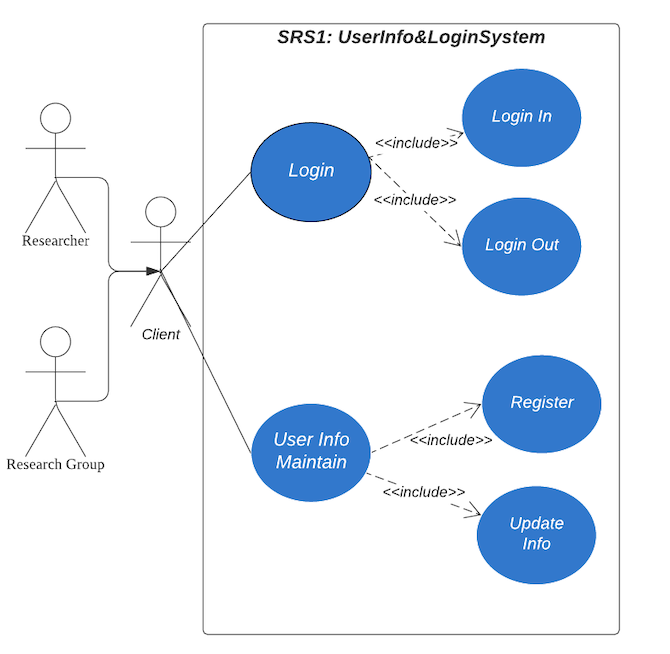
\includegraphics[width=7cm]{./img/SRS1.png}}
	% \hspace{0.5cm}
	\subfloat[Use Case Sub-Req 2]{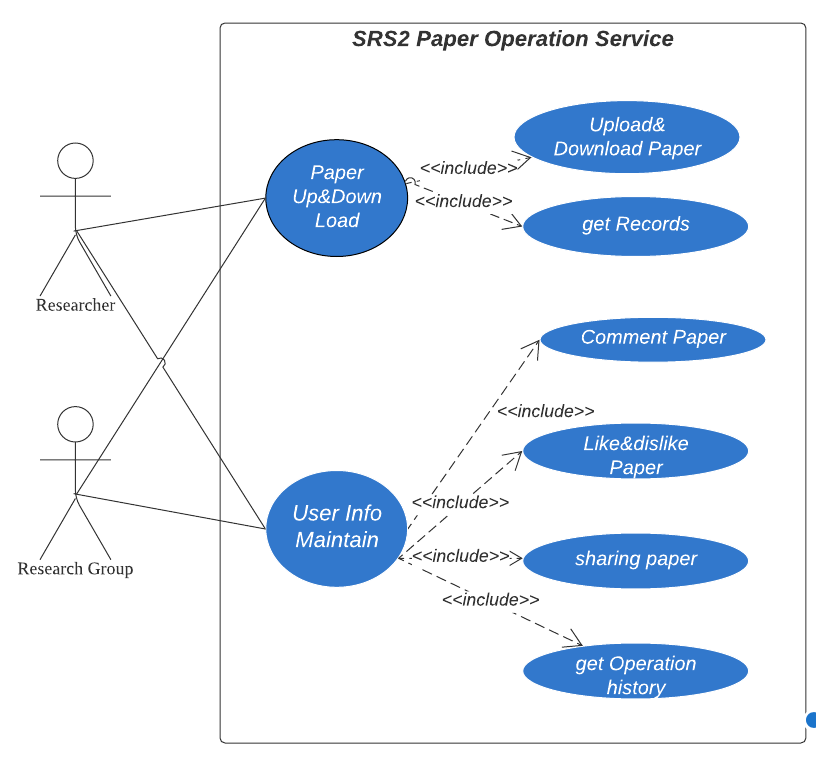
\includegraphics[width=7cm]{./img/SRS2.png}}

	\subfloat[Use Case Sub-Req 3]{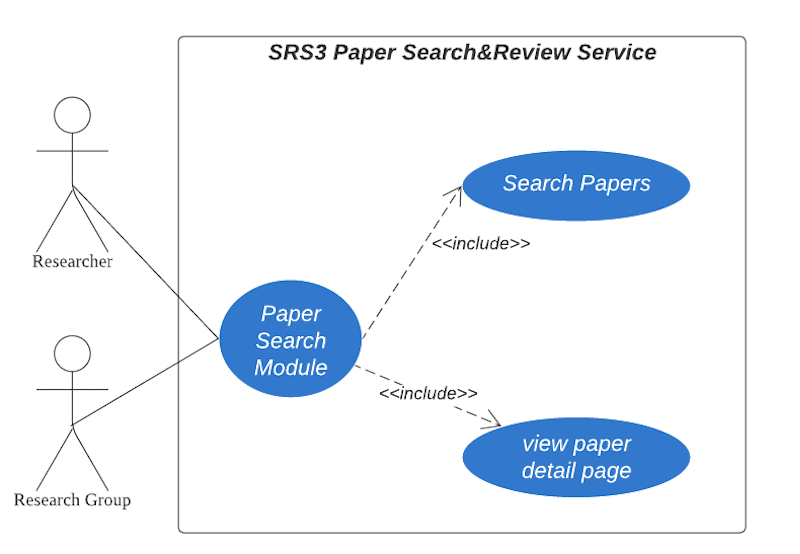
\includegraphics[width=7cm]{./img/SRS3.png}}
	\caption{Use case Diagrams}\label{fig:subusercases-1}
\end{figure*}

\begin{figure*}[!ht]
	\centering

	\subfloat[Use Case Sub-Req 4]{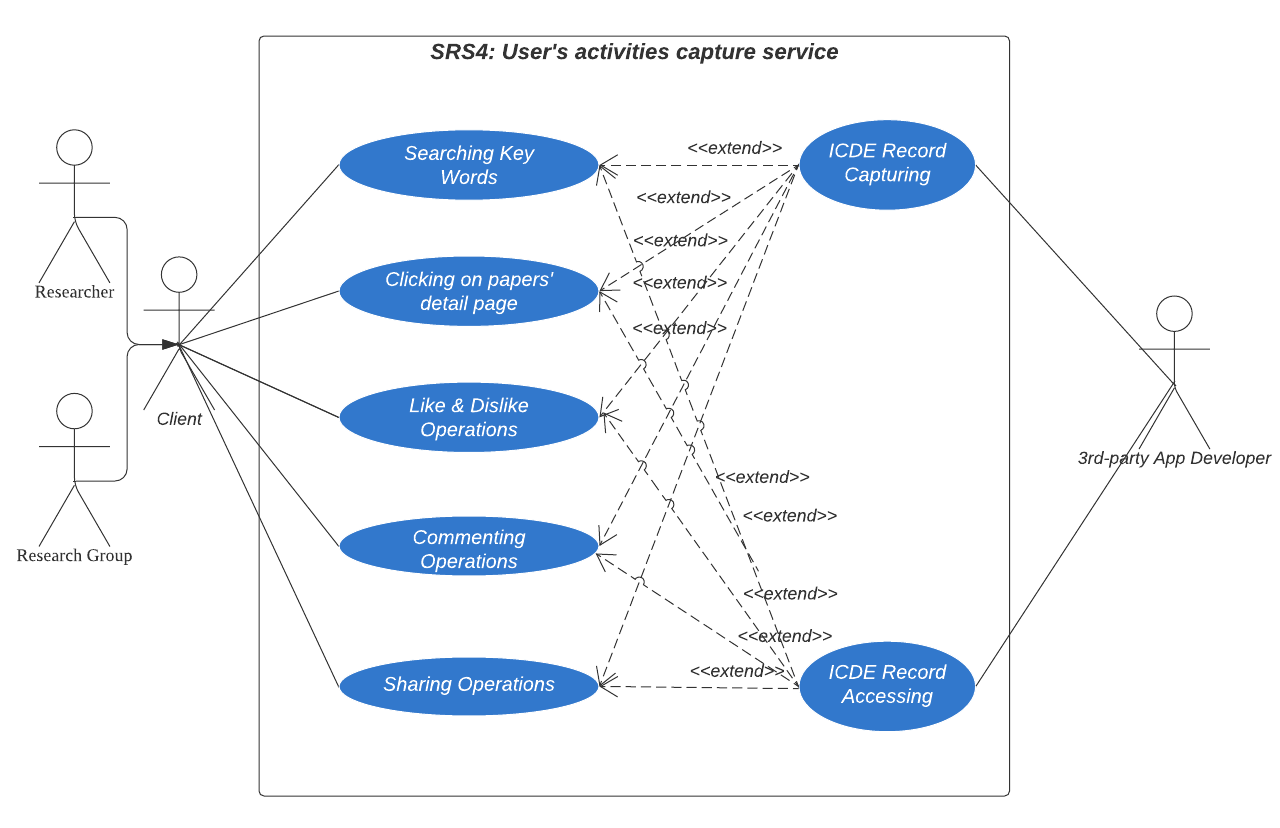
\includegraphics[width=7cm]{./img/SRS4.png}}
	% \hspace{0.5cm}
	\subfloat[Use Case Sub-Req 5]{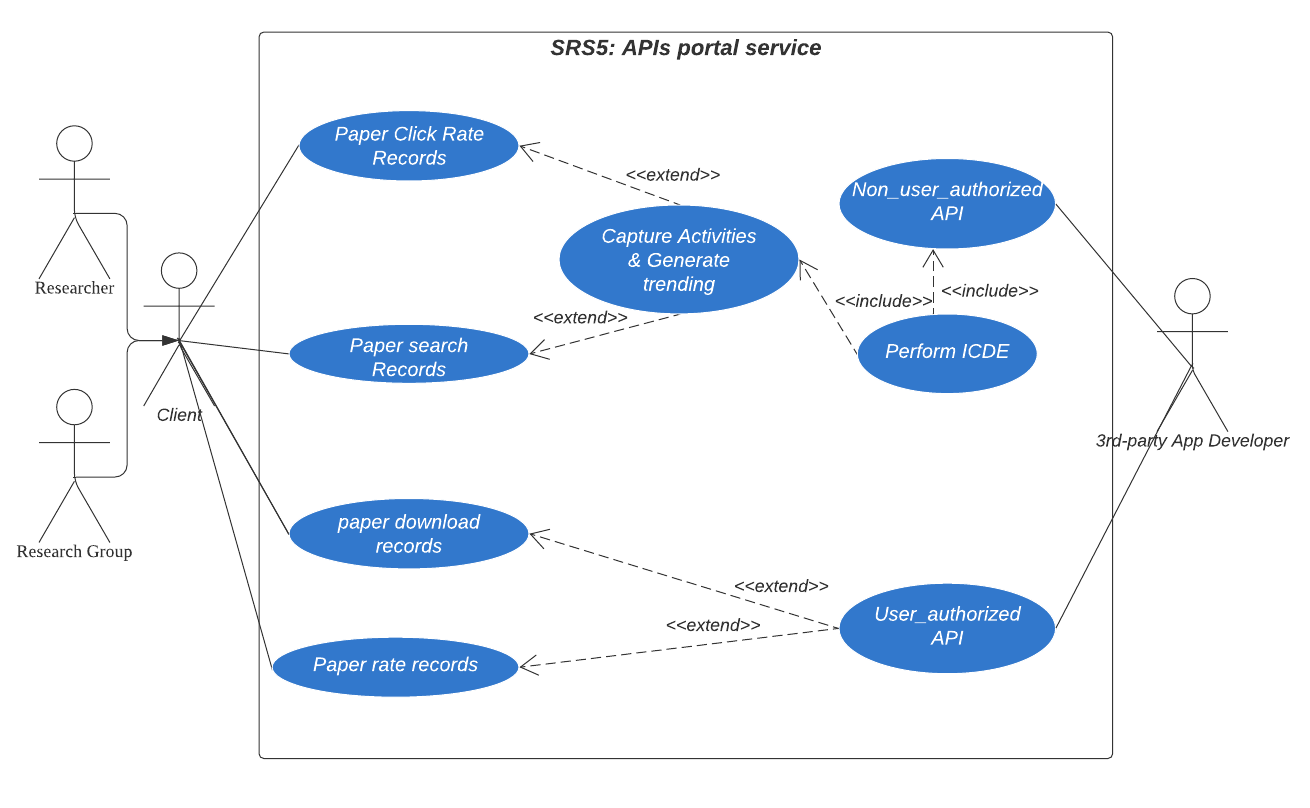
\includegraphics[width=7cm]{./img/SRS5.png}}

	\subfloat[Use Case Sub-Req 6]{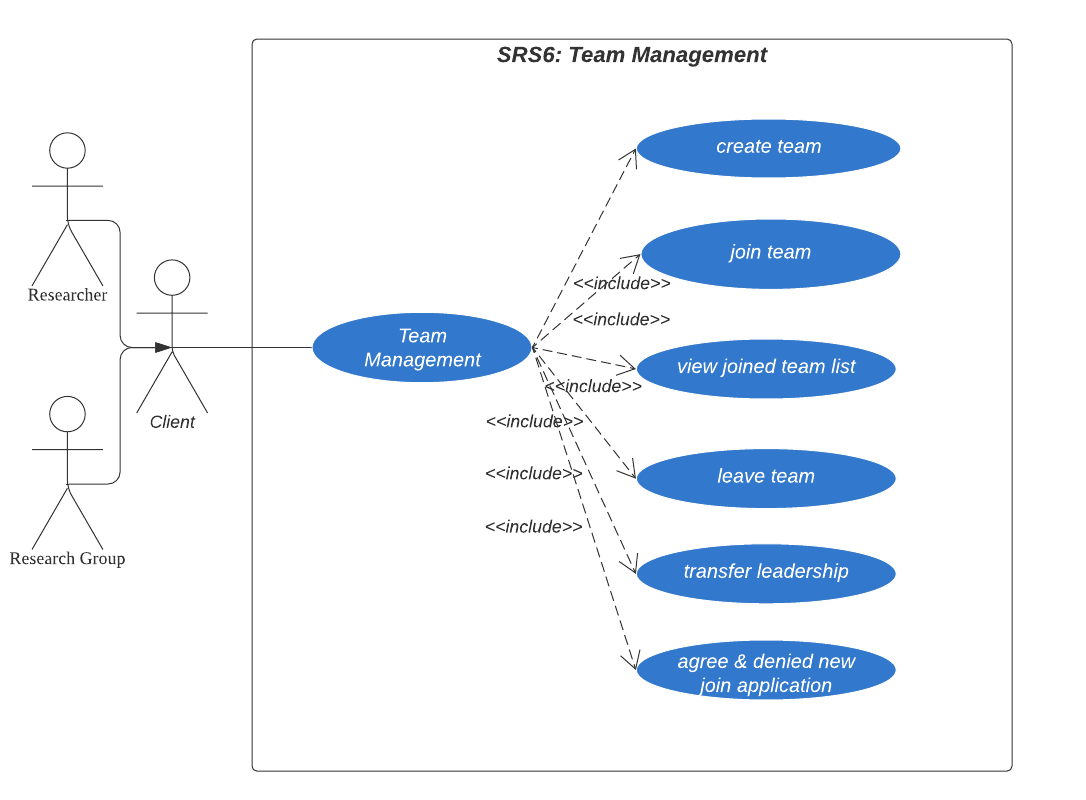
\includegraphics[width=7cm]{./img/SRS6.png}}
	% \hspace{0.5cm}
	\subfloat[Use Case Sub-Req 7]{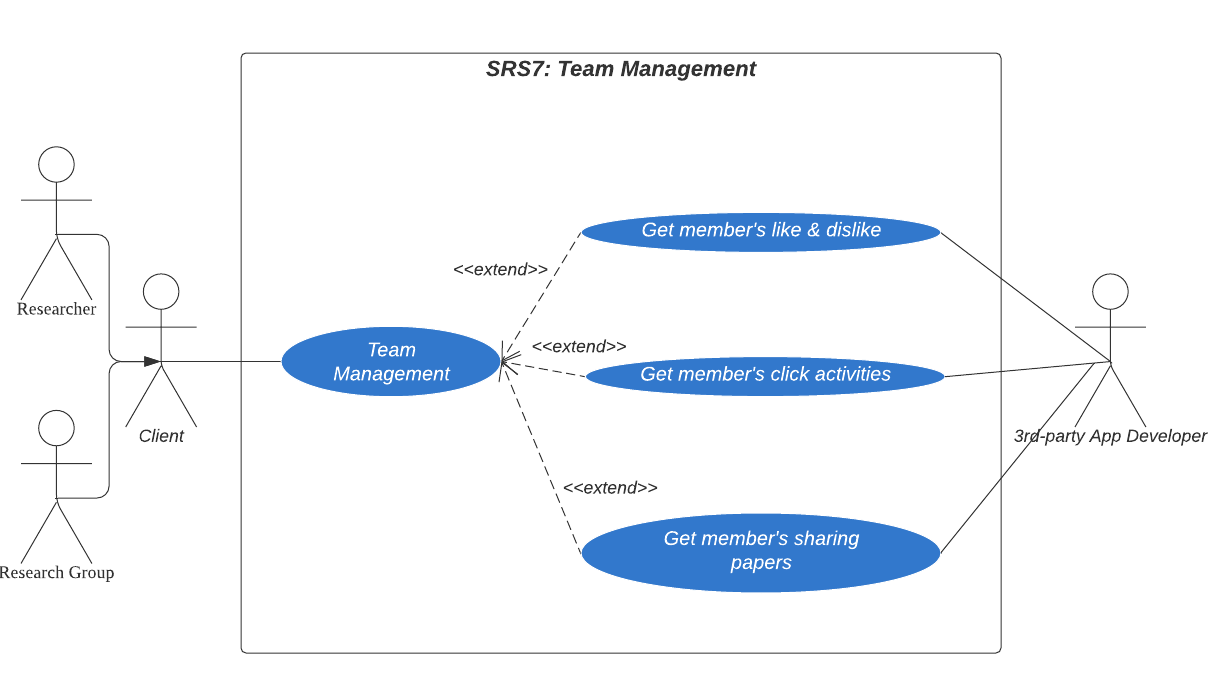
\includegraphics[width=7cm]{./img/SRS7.png}}

	\caption{Use case Diagrams}\label{fig:subusercases-2}
\end{figure*}

% import outer tex
\import{.}{sys-arch.tex}

% import outer tex
\import{.}{sys-modeling.tex}

\import{.}{sys-ui-prototype}

\section{Repeat Req2 and Further evaluate the process and milestones}

After attending Week 7 Lecture our team found that we shall adding the non-functional
requirement for our system that constraints on the services offered by the system.
We consider timing constraints that limit the whole service hours for users including
research individual and research group. During 0:00 to 6:00 on every Sunday the system
will unavailable for researchers(either the individual or the group).
% We repeat requirement 2 as following documentation \ref{fig:newreq}.

% \begin{figure}[htp]
% 	\centering
% 	% \subfloat[1.Class Diagram,  2.Statement Diagram,  3.Use Case ]{
% 	% 	\begin{minipage}{\linewidth}
% 	% 		\includegraphics[width=0.3\linewidth, height = 0.15\textheight, keepaspectratio=true]{class new.png}
% 	% 		\includegraphics[width=0.3\linewidth, height = 0.15\textheight, keepaspectratio=true]{statements_new.png}
% 	% 		\includegraphics[width=0.4\linewidth, height = 0.2\textheight, keepaspectratio=true]{use case new.png}
% 	% 	\end{minipage}}
% 	% \subfloat[4.Activities Diagram,  5.Sequence Diagram]{
% 	% 	\begin{minipage}{\linewidth}
% 	% 		\includegraphics[width=0.4\linewidth, height = 0.2\textheight, keepaspectratio=true]{activities new.png}
% 	% 		\includegraphics[width=0.4\linewidth, height = 0.2\textheight, keepaspectratio=true]{sequence new.png}
% 	% 	\end{minipage}}
% 	\subfloat[Class Diagram]{\includegraphics[width=5cm]{./img/class new.png}}
% 	\subfloat[State Diagram]{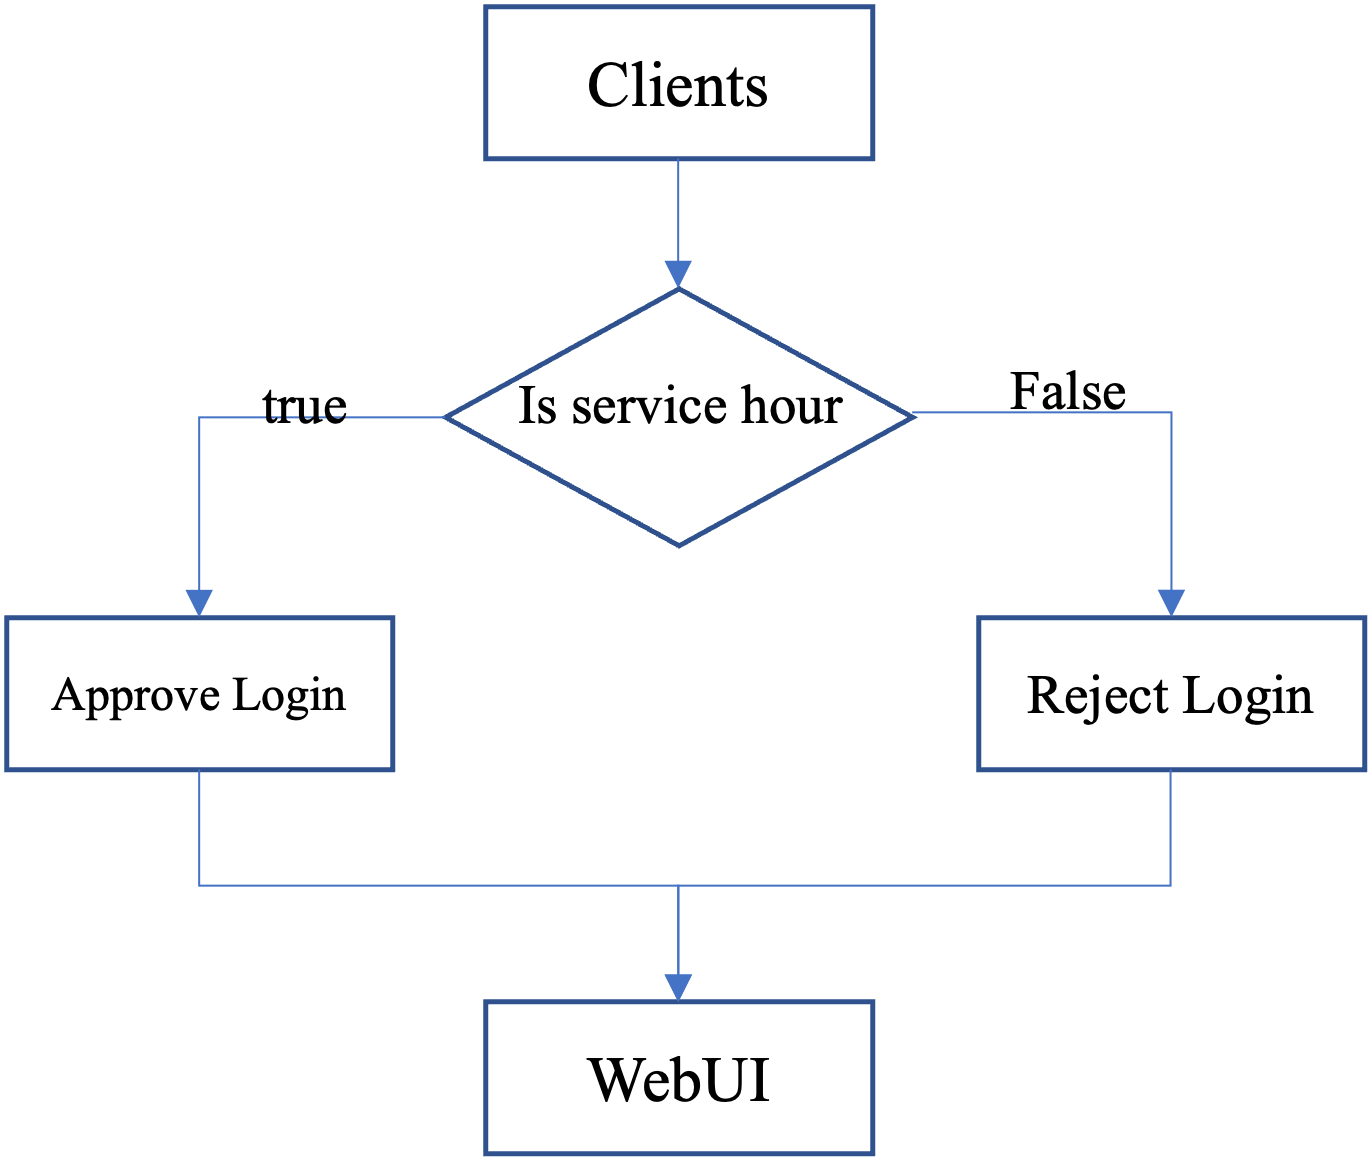
\includegraphics[width=5cm]{./img/state_new.png}}

% 	\subfloat[Activities Diagram]{\includegraphics[width=5cm]{./img/activities new.png}}

% 	\subfloat[Use Case]{\includegraphics[width=5cm]{./img/use case new.png}}
% 	\subfloat[Sequence Diagram]{\includegraphics[width=5cm]{./img/sequence new.png}}

% 	\caption{Documentation for new requirement}
% 	\label{fig:newreq}
% \end{figure}

The whole process and milestones are newly evaluate and listed the milestone in Jira as Figure \ref{fig:roadmap}.
Currently we have finished Sprint1 and the sub-tasks are listed on Jira as Figure \ref{fig:sprint1}.
The schedule for team is that 8 hours per member per week, and the budget is keeping stable.

\begin{figure*}[htp]
	\centering
	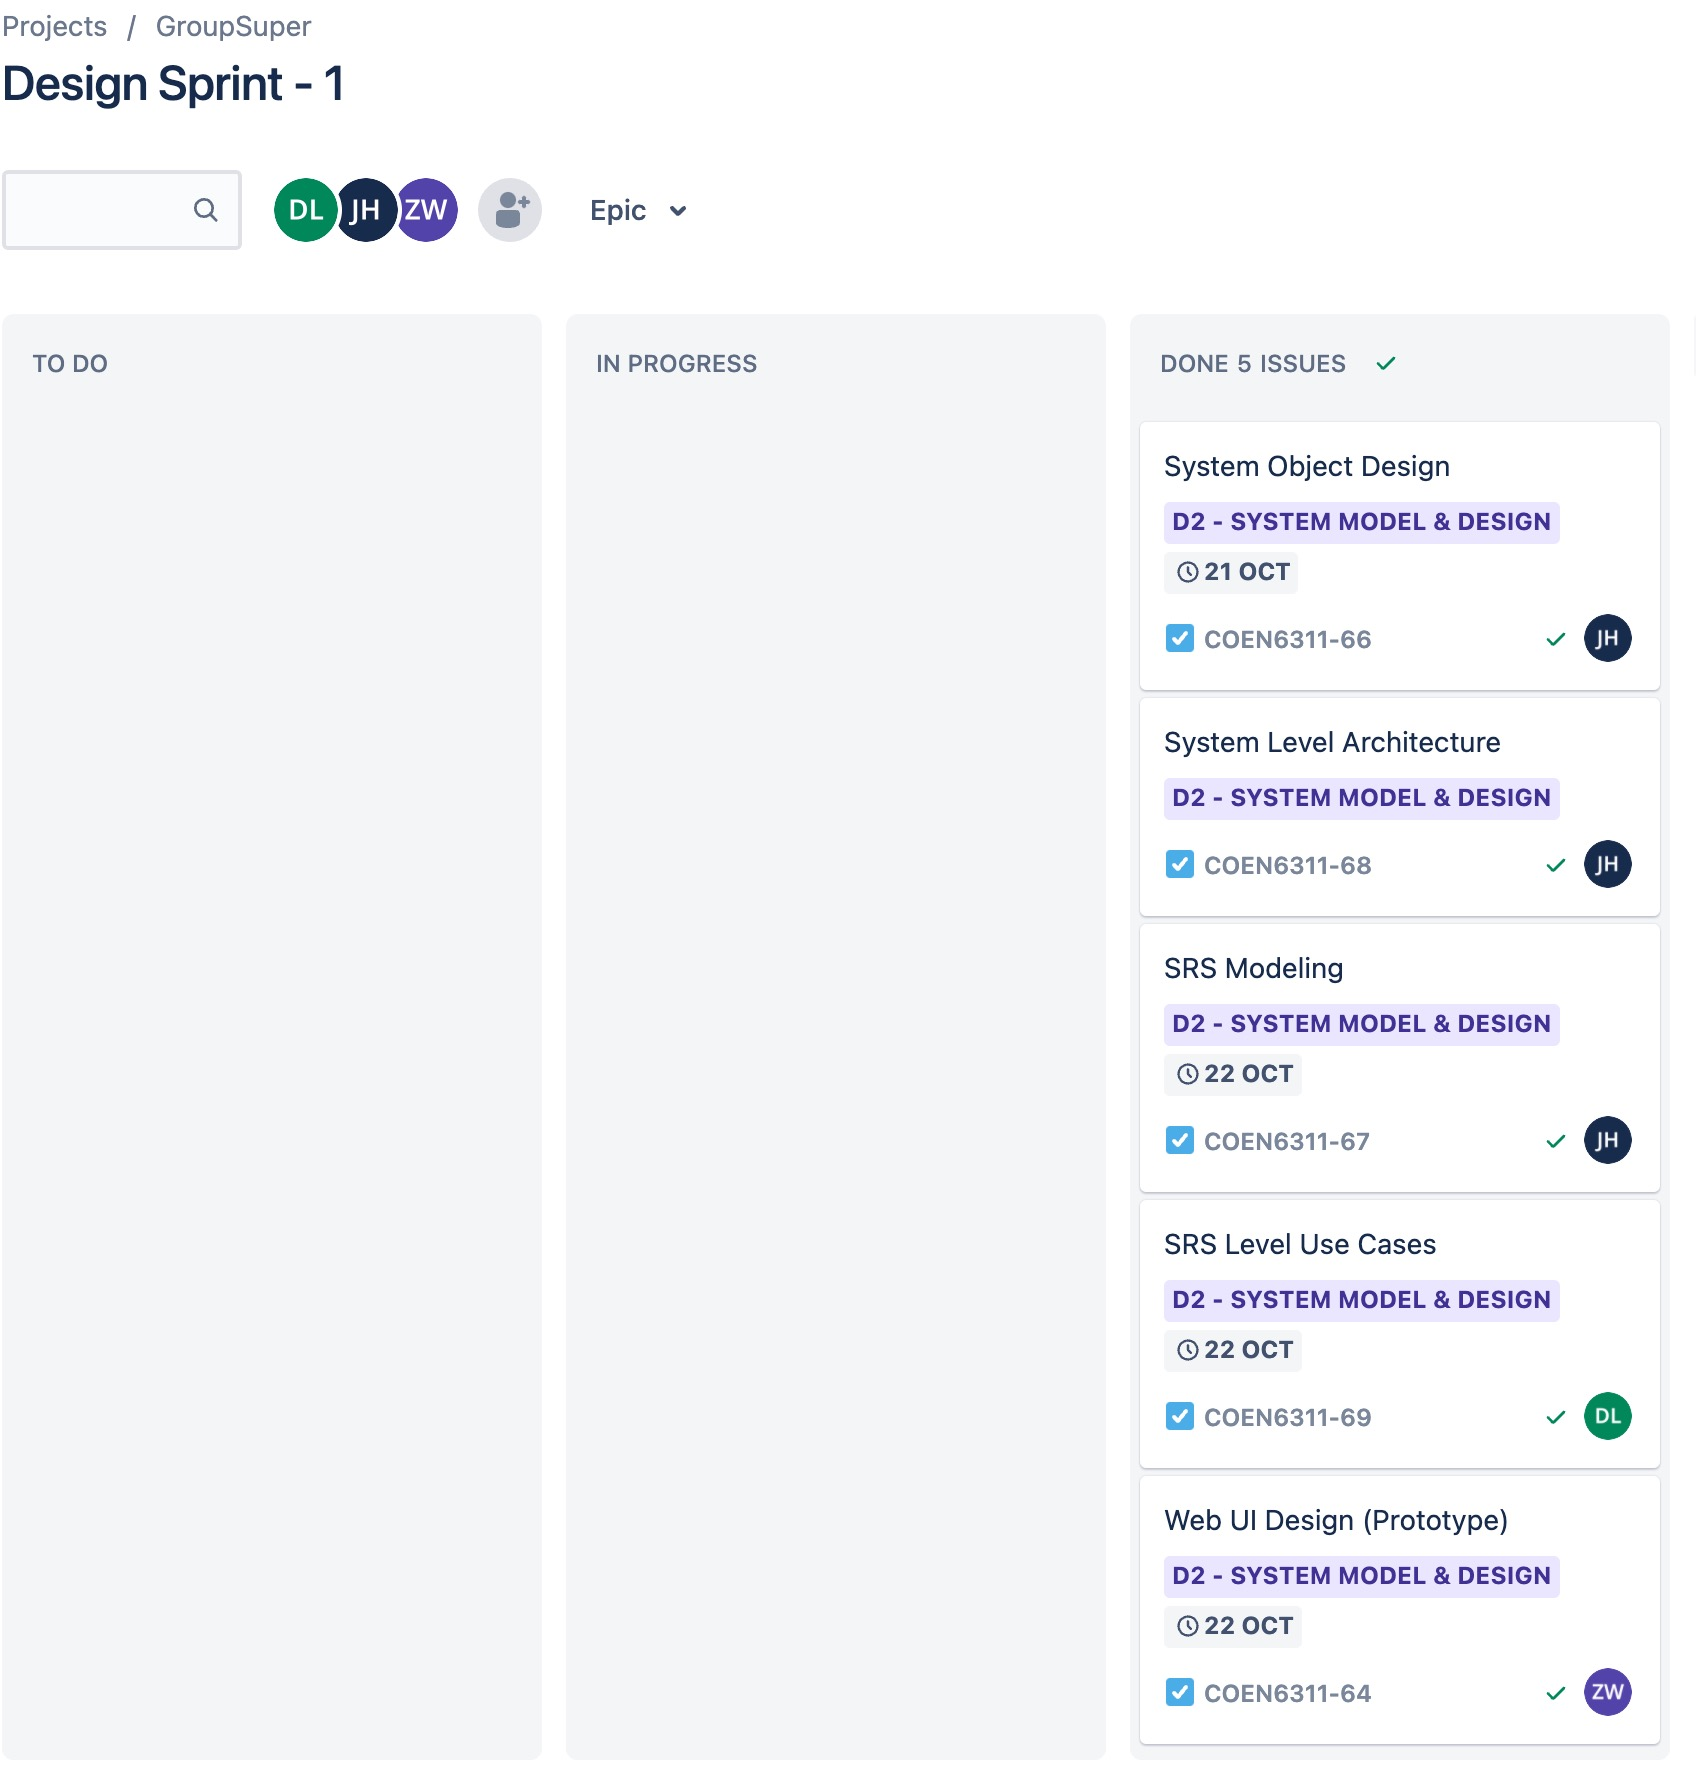
\includegraphics[scale=0.14]{./img/Sprint1.jpg}
	\caption{Sprint1 Sub-tasks on Jira}
	\label{fig:sprint1}
\end{figure*}

% \bibliographystyle{ACM-Reference-Format}
% \bibliography{sample}
\end{document}
\endinput
